\chapter{Implementation}\label{ch:implementation}
Our editor is implemented as a plugin for the 3D modeling software \textit{SketchUp}. Our system is composed of an Editor, which can place truss primitives and physics components and modify created structures, a physics simulation, which can calculate forces and movement interactively, and an export component, which translates the object in the editor into 3D printable files. The main goal of our plugin is to create dynamic truss structures. Our plugin supports the user in the creation of large-scale dynamic objects by visualizing the forces acting on the object, while the user can move the object interactively. It can also create animations that play automatically, warning users if the forces during the animation exceed the force limits of the structure and helping them in finding a better approach. Furthermore, it aids the user in finding the most efficient movement layout in the complex truss structure.\\
The user interface is implemented in JavaScript, using the node.js framework for advanced features. The connection to SketchUp and most functionalities are written in Ruby. The physics simulation is based on a C++ physics engine, using a Ruby wrapper to embed it in our code base.\\
After explaining the architecture, this chapter will demonstrate the tools and functionalities in greater detail and explain the underlying components.

\section{Architecture}
The software can be divided into four components. The most user-facing one is the TrussFormer Editor. It contains the user interface and the construction functionalities. The other components can be seen as extensions to the editor. The \textit{Force Analysis} calculates tension force on the created structure. The tensions forces are calculated using an adapted version of the \textit{MSPhysics}\footnote{https://extensions.sketchup.com/en/content/msphysics} physics engine, which is a Ruby wrapper around the C++ physics engine \textit{NewtonDynamics}\footnote{http://newtondynamics.com/forum/newton.php}.\\
This physics engine is also used by another component, the \textit{Export Functionality}. It uses the physics features to detect changing angles between Edges, indicating the need for a hinging hub.
\begin{figure}[!h]
    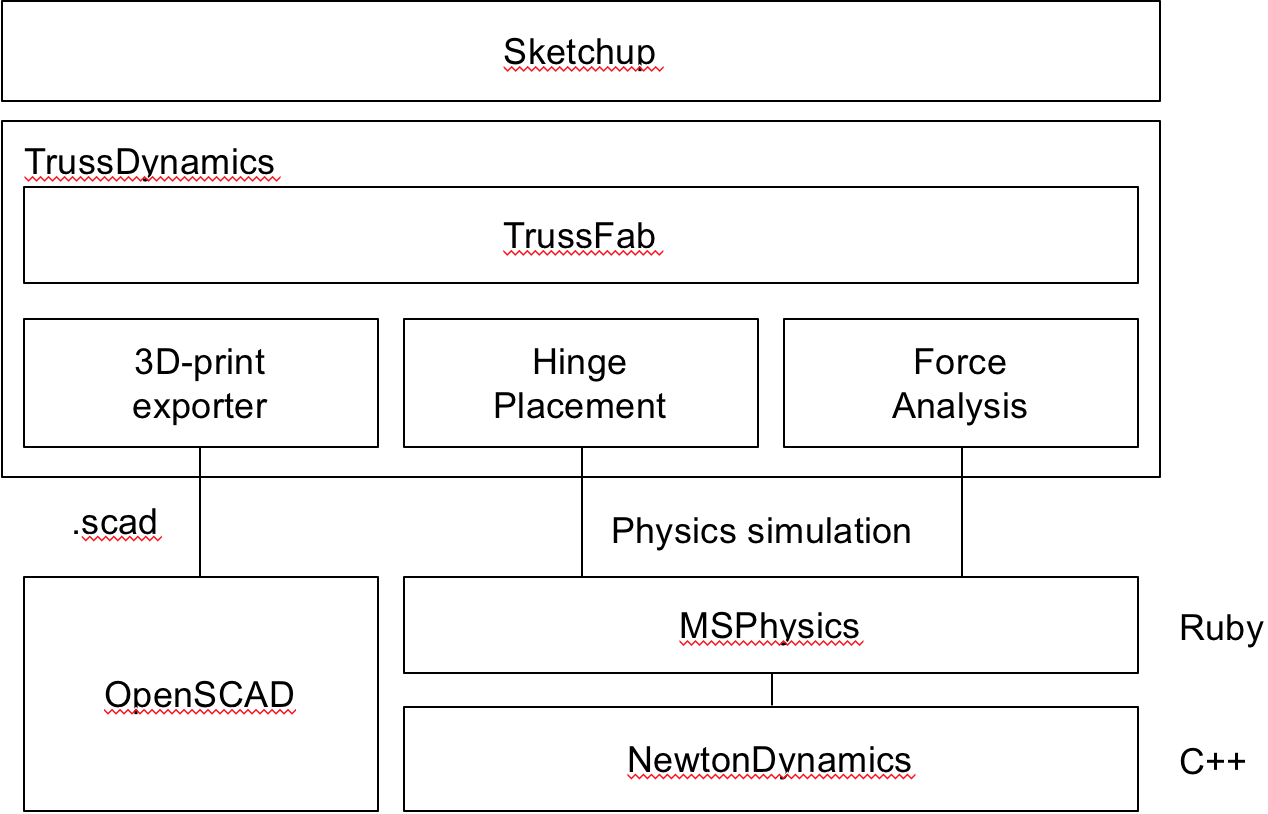
\includegraphics[width=\textwidth]{Implementation/TrussFormer_Architecture_Overview.png}
    \centering
    \caption{TrussFormer Architecture}
    \label{fig:architecture}
\end{figure}
The structure diagram in figure \ref{fig:architecture} shows how the components fit into our system. Details for each component will be explained later in this chapter.

All components are stored in a graph structure. The building parts are \textit{Edges}, \textit{Nodes} and \textit{Triangles}. They all inherit \textit{GraphObject}. The purpose of these objects is providing user-facing functionalities and storing lower-level components. An overview of the graph structure can be seen in \ref{fig:graph}.\\
The \textit{Graph} is implemented as a Singleton \improvement{explain what a Singleton is} that stores and provides access to all GraphObjects, creates new ones and provides convenience functions for user interactions, such as finding the node closest to the mouse cursor. As this class is a singleton, every module of the software has access to the objects.\\
Each of these objects has access to its underlying logic-bearing component, called \textit{SketchupObject}.\improvement{Clarify. Either explain what that means (Hubs, Links, Surfaces) or at least have a forward reference} The access to this functionality is, however, not implemented in this superclass, but in each subclass, having the specific name as an accessor. This design decision was made to improve code readability, and decrease coding errors caused by accessing the wrong SketchupObject.\improvement{Show before and after code snippet}\\
\begin{figure}
    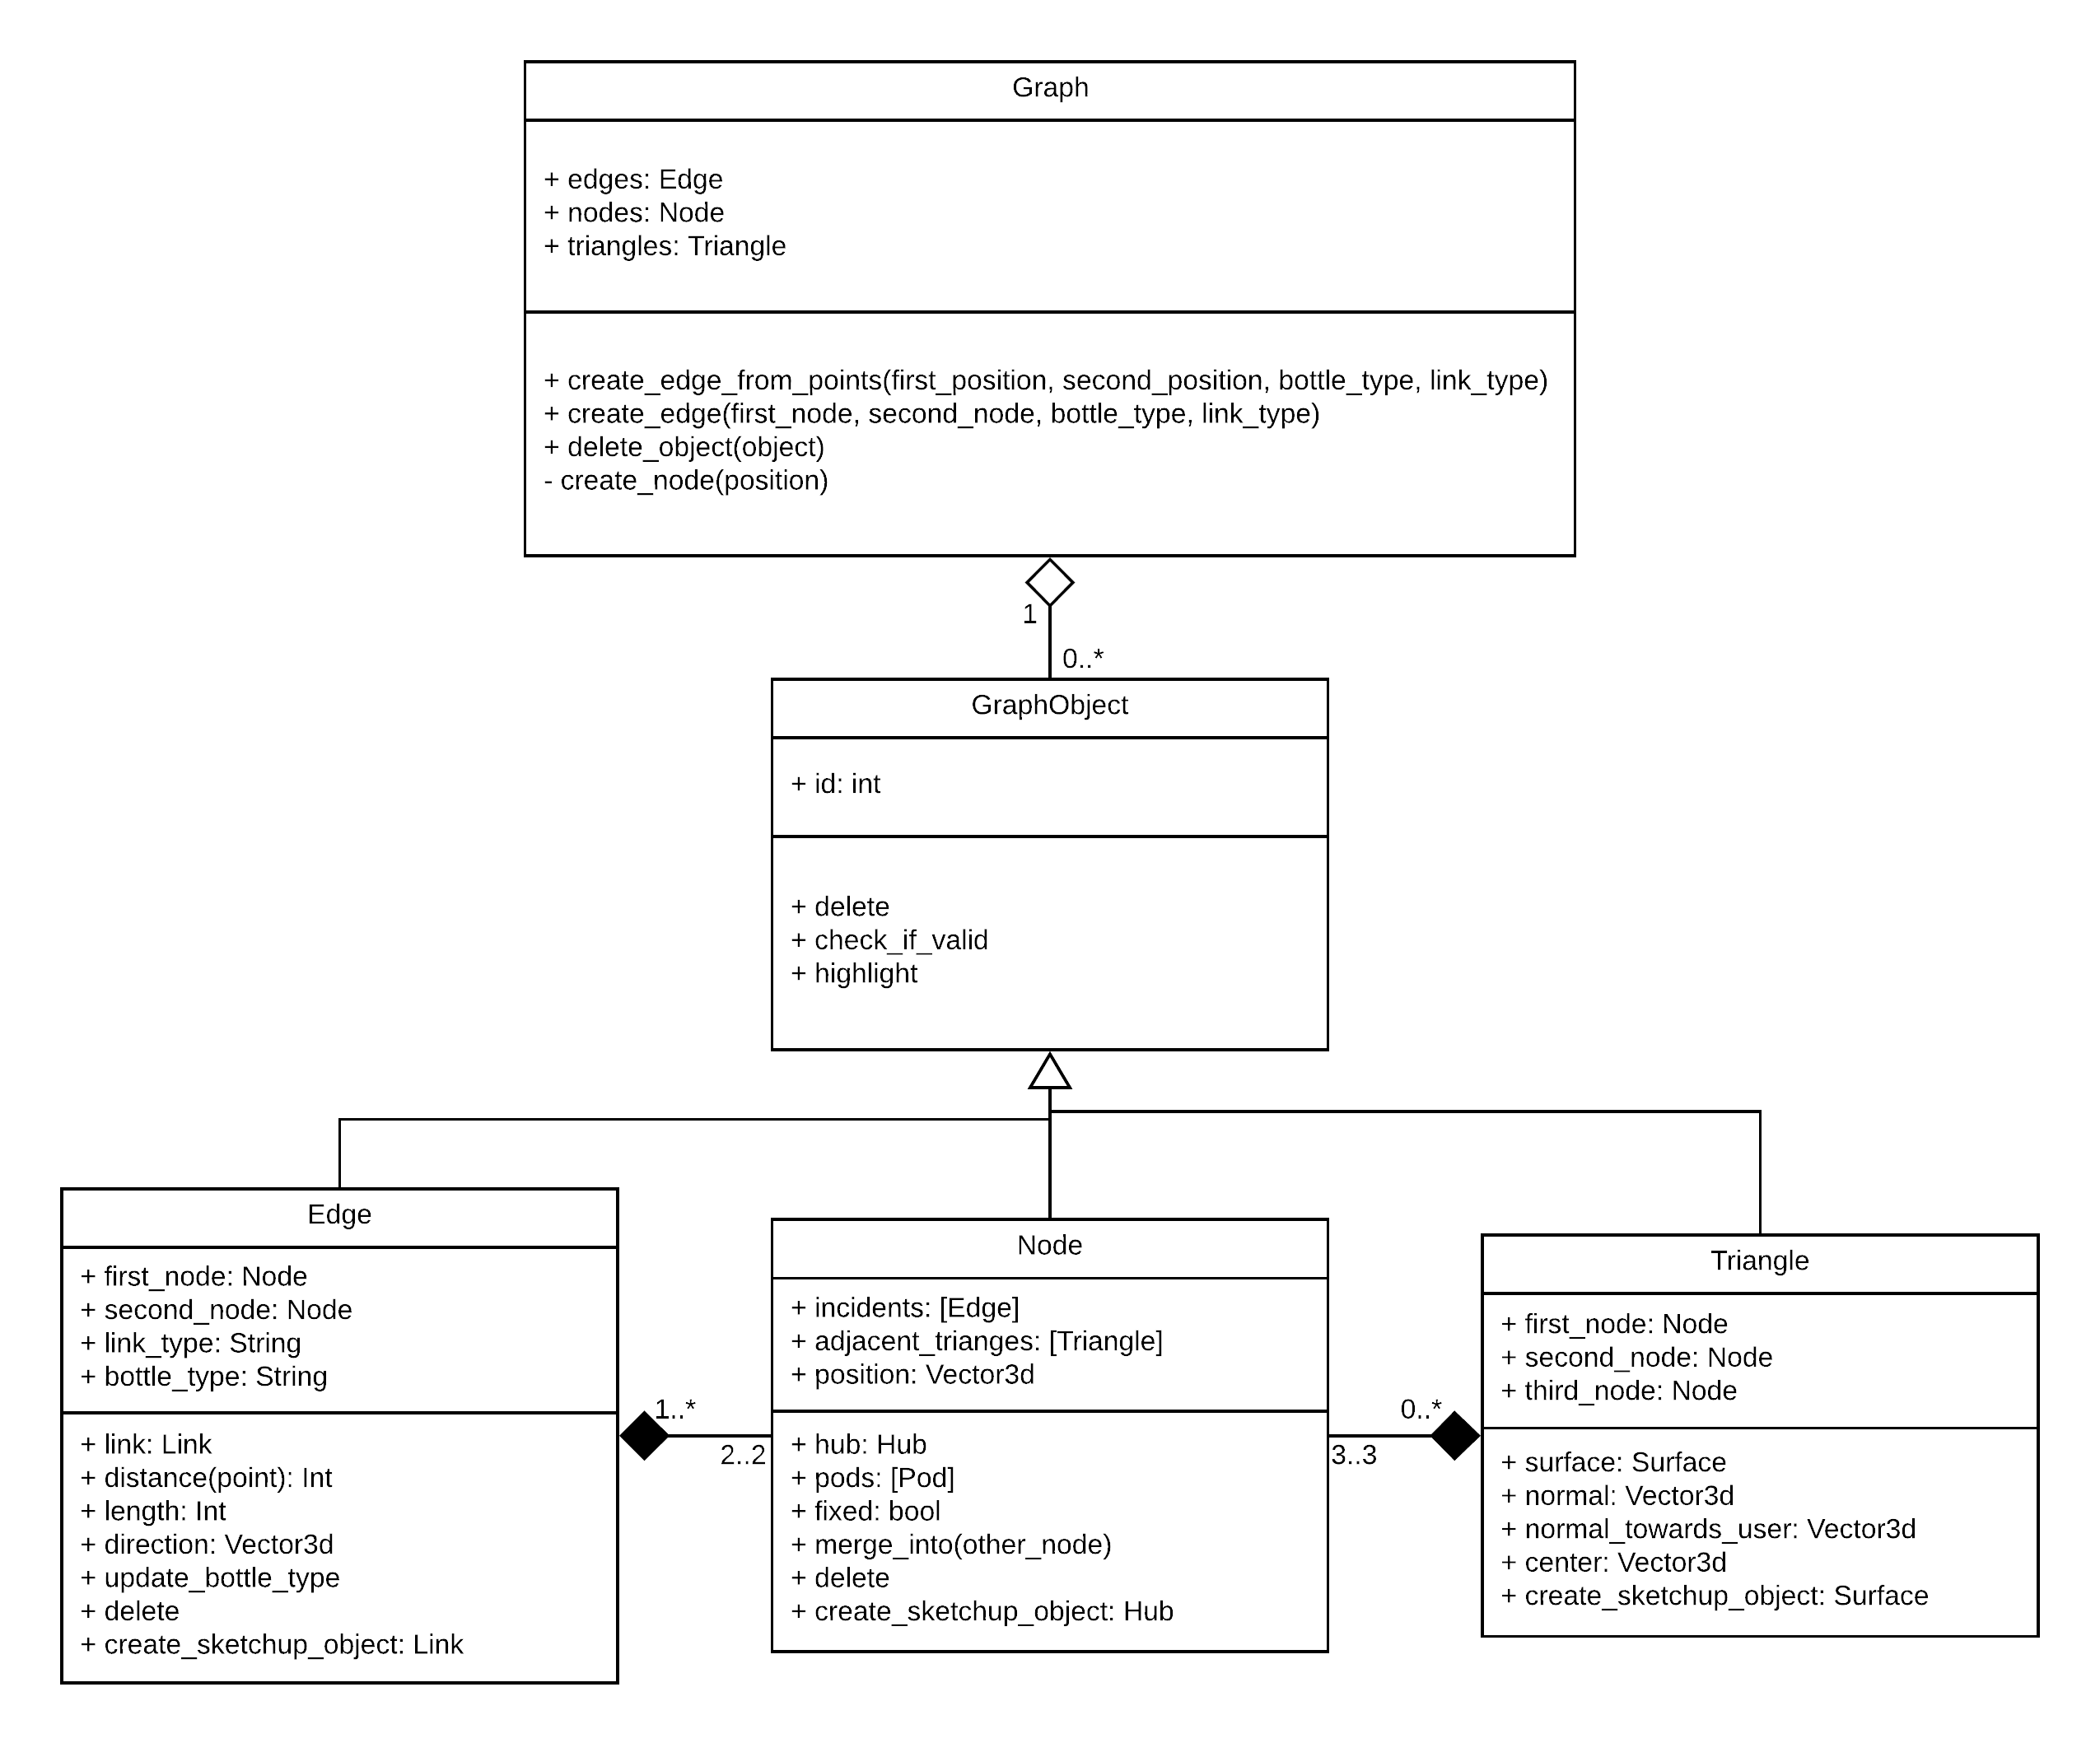
\includegraphics[width=\textwidth]{Implementation/TrussFormer_Graph.png}
    \centering
    \caption{Class Diagram showing the high-level Graph Structure of the TrussFormer Designer}
    \label{fig:graph}
\end{figure}
The responsibility of the GraphObject class is primarily unifying the way the appearance in SketchUp of the underlying object can be changed as much as possible. This includes highlighting a specific object if the mouse hovers over it, resetting the object to its default state and creating and deleting it. More complex methods need to be implemented in the respective subclass.\\
\textit{Nodes} are the connecting components of the structure. \textit{Edges}, as well as \textit{Triangles} are created based on Nodes. Apart from storing adjacent Edges and Triangles, a Node can specify their positions in the SketchUp world. The Nodes' adjacent objects constantly check if their position has changed and update their SketchUp representation accordingly. If the structure is deformed in such a way that a Node will be at the same position as another one, the Node object can automatically merge into the other Node. The Node will iterate over all its adjacent Edges and tell each one, apart from the Edges that run from the other Node to the Edge the Node is hinging around (i.e. the Edge that is opposite the Node), to exchange itself with the Node it wants to merge into. These Edges are removed from its own adjacent Edges and added to the collection of the new Node. The same happens for all adjacent Triangles. As a last step, the Node deletes itself and all remaining adjacent Edges and Triangles (which will be the Edges and Triangles that got merged). The object will then be adapted according to the new positions using the \textit{Relaxation algorithm}, described in section \ref{sec:relaxation}.
\clearpage
\begin{lstlisting}[language=Ruby, label={lst:merging_code}, caption=Merging of two Nodes]
  def merge_into(other_node)
    merged_incidents = []
    @incidents.each do |edge|
      edge_opposite_node = edge.opposite(self)
      next if other_node.edge_to?(edge_opposite_node)
      edge.exchange_node(self, other_node)
      other_node.add_incident(edge)
      merged_incidents << edge
    end
    @incidents -= merged_incidents

    merged_adjacent_triangles = []
    @adjacent_triangles.each do |triangle|
      new_triangle = triangle.nodes - [self] + [other_node]
      next unless Graph.instance.find_triangle(new_triangle).nil?
      triangle.exchange_node(self, other_node)
      other_node.add_adjacent_triangle(triangle)
      merged_adjacent_triangles << triangle
    end
    @adjacent_triangles -= merged_adjacent_triangles

    delete
  end
\end{lstlisting}
Another component that is tightly coupled to Nodes are \textit{Pods}. A Pod acts as a stand for the object and tells TrussFormer that this Node should not change its position.\todo{add image}\\
The \textit{Edges} are the most visual components of TrussFormer. They are visualized by bottles of different lengths, if they are static links, or as two cylinders forming an actuator, if they can have variable lengths. The Edges handle creating the correct model and changing it if the user decides to place a different kind of Edge. Edges play a big role in the simulation.
The last high-level component in TrussFormer is the \textit{Triangle}. A Triangle is primarily used as a convenient access to multiple Nodes or Edges. Most tools that work on Nodes, such as the \textit{Add Weight Tool}, can also be applied to Triangles, adding weight to all three connected Nodes. The Triangle also provides functions for telling the \textit{MouseInput} in where a certain face is directed.\improvement{IMPROVE!}

\subsection{SketchupObjects}
As mentioned before, each GraphObject contains a lower-level \textit{SketchupObject}. These objects are responsible for more complex, lower-level tasks, such as physics calculations, rendering and communication to the simulation engine.\\
Each SketchupObject has a \textit{Sketchup::Entity}, which is a class provided by SketchUp that is capable of handling the representation in SketchUp itself. This includes changing the color of the model, hiding and transforming. On creation, each SketchupObject is also persisted in the entity\todo{find out why exactly I did that}.
\begin{figure}[h!]
    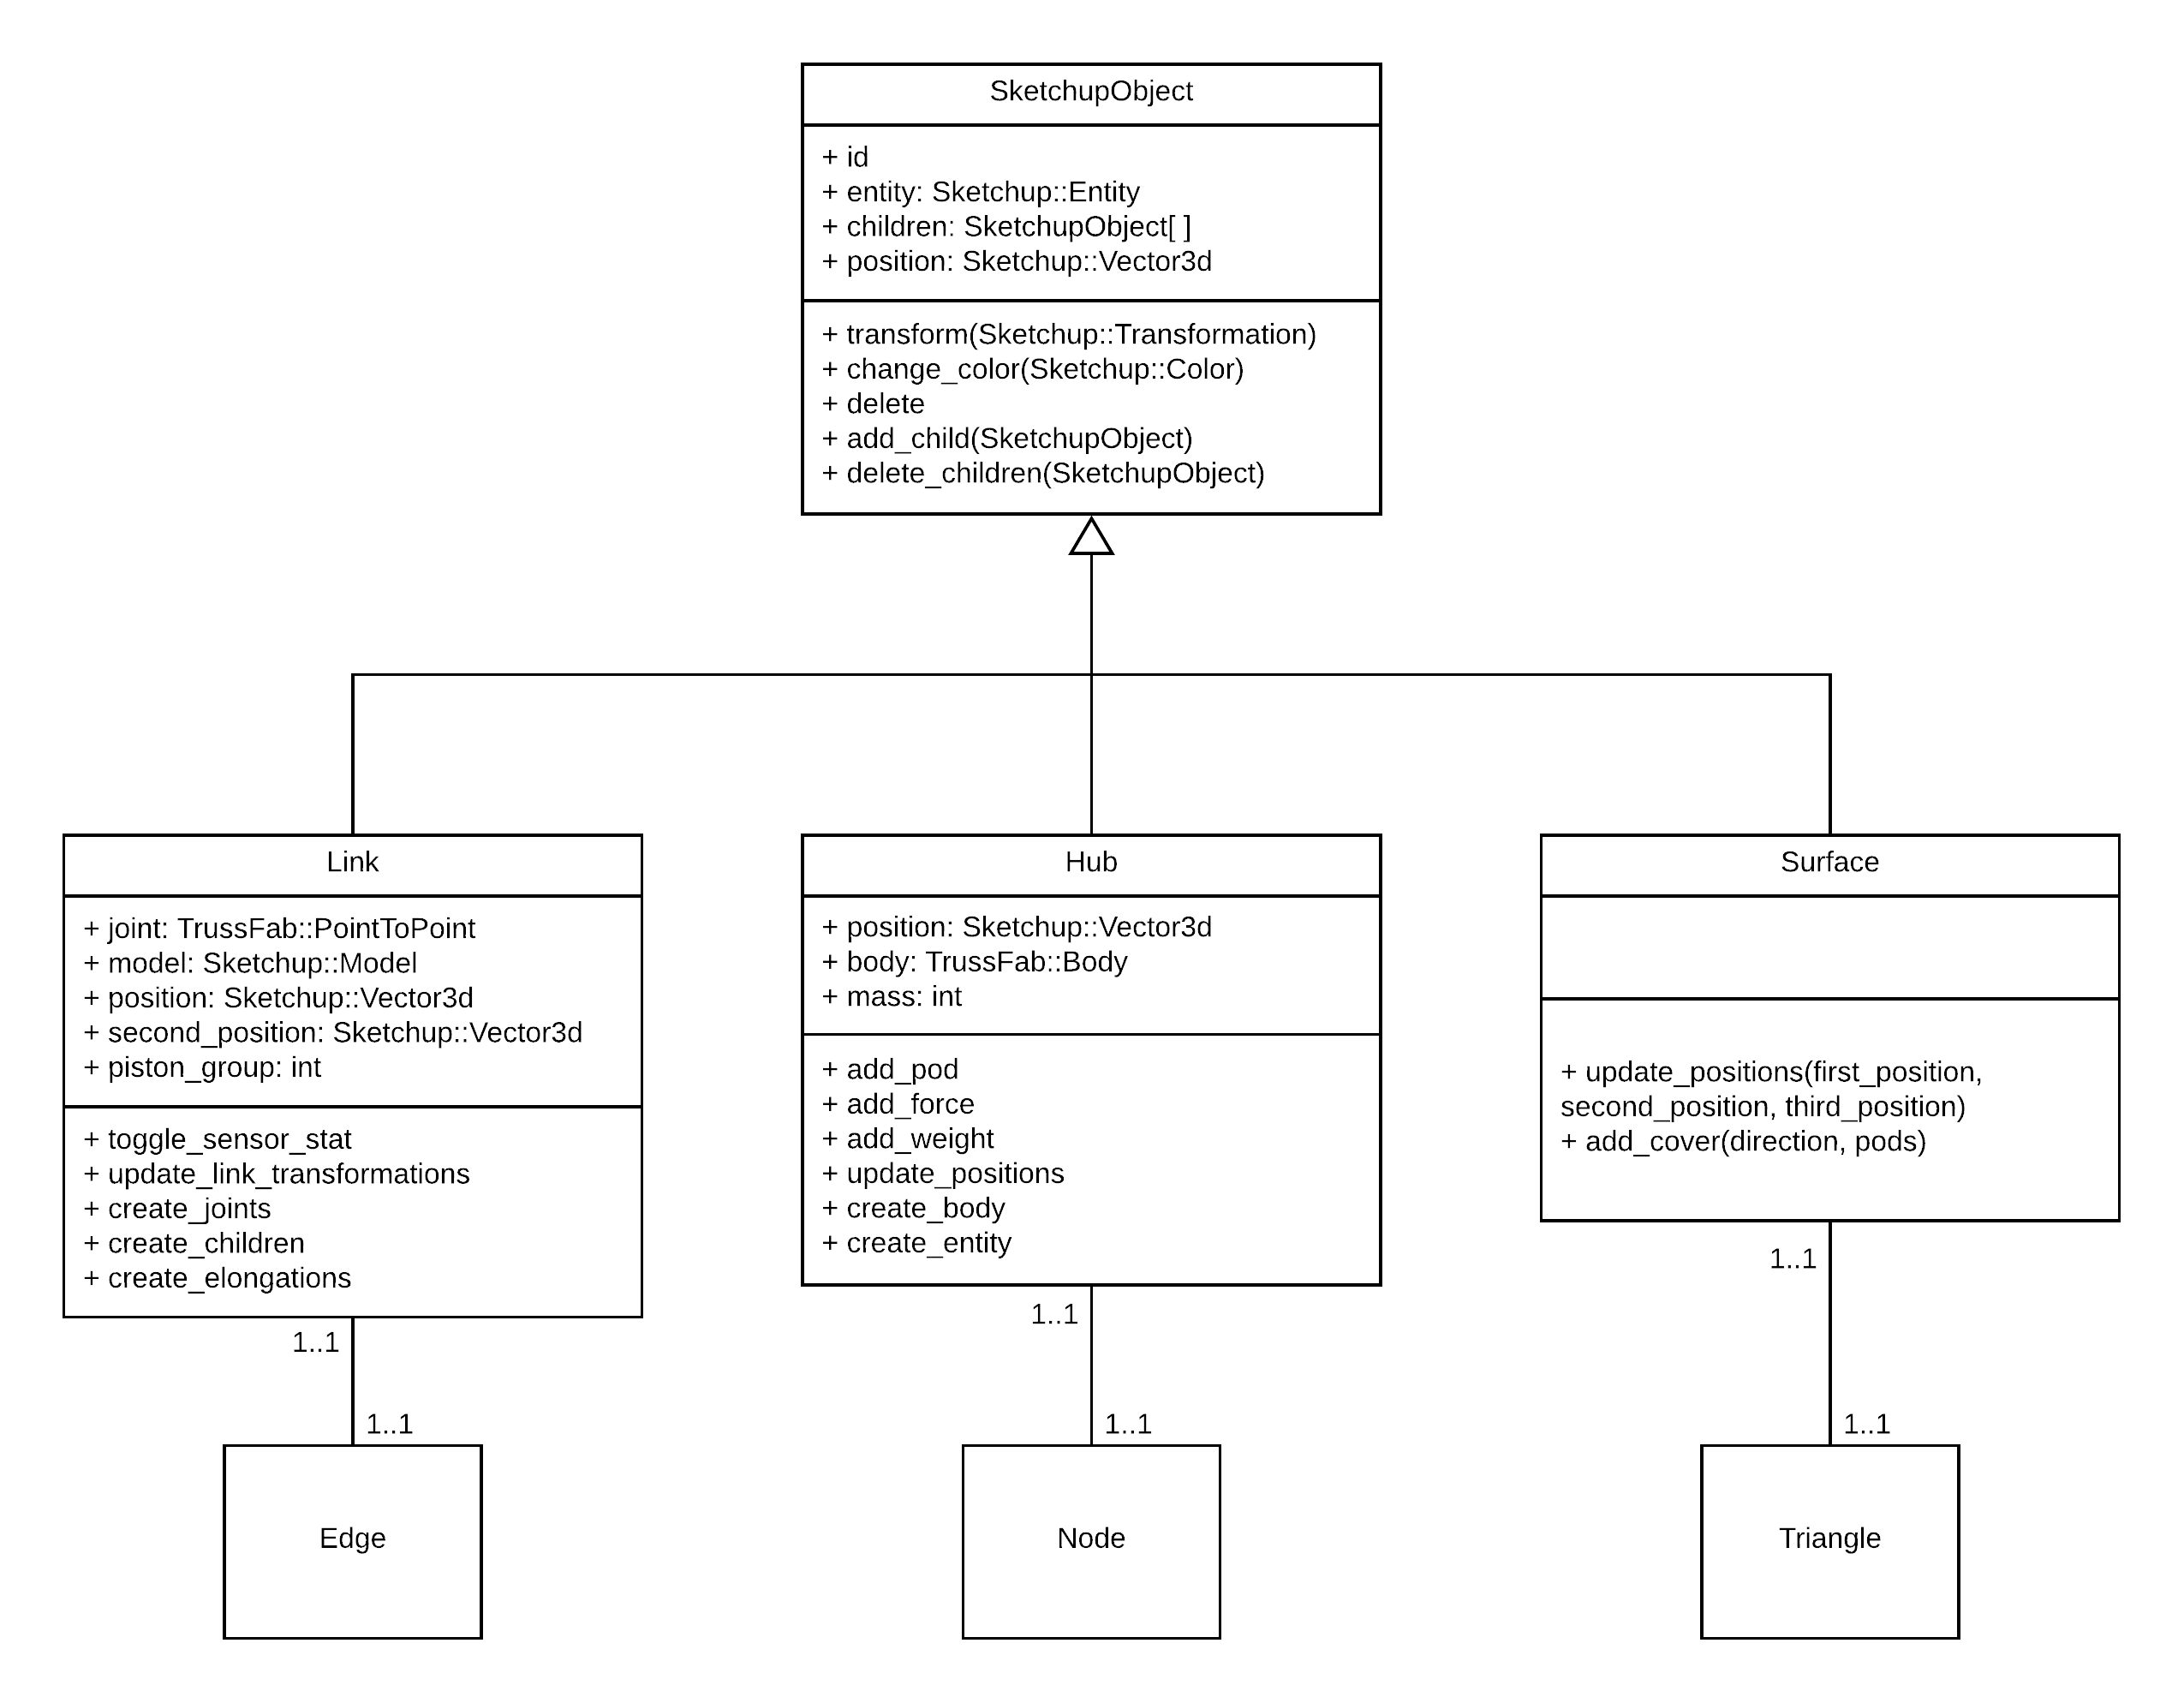
\includegraphics[width=\textwidth]{Implementation/TrussFormer_SketchupObjects.png}
    \centering
    \caption{Class Diagram showing the UI components of the graph structure}
    \label{fig:sketchup_objects}
\end{figure}

\subsubsection{Hubs}
\textit{Hubs} are the underlying structures used by Nodes. For ease of calculation and increased performance of the \textit{Simulation} (s.a. section \ref{sec:simulation}), only the Hubs of a structure have physical properties. Hubs therefore have to store information about the object, such as the weight. The weight is calculated based on the number of bottle links and actuators connected to this node. For our system, we measured these values empirically by taking the weight of a screw and half the weight of a bottle link or an actuator per connection and adding it to the average weight of an empty printed hub. The \textit{add weight} and \textit{add force} tools will additionally increase this value, while the Hub also displays the indicators for these tools.\\
These values, together with a few other variables, then form the basis of our simulated structure.

\subsubsection{Links}
\textit{Links} define the connection between two hubs. They are tightly coupled to the physics engine and contain the \textit{Joints}, which are objects used by the engine itself. Available joints are:
\begin{itemize}
    \item TrussFormer::PointToPoint - A static connection between two points
    \item TrussFormer::PointToPointActuator - A variable-length connection between two points
    \item TrussFormer::PointToPointGasSpring - A variable-length connection between two points with a distance-based force factor
    \item TrussFormer::GenericPointToPoint - A variable-length connection between two points with a custom force factor
\end{itemize}
The Link is therefore responsible for defining the distance between two Hubs. Because of the nature of truss structures, this can have impact on the whole object and create the variable geometry truss. Joints will be discussed in more detail in the simulation section \ref{sec:simulation}.

\subsubsection{Surface}
The \textit{Surface} is primarily used to visualize what face of the truss the user is currently selecting, by changing the color between three bottles. It can also hold a cover, which has mainly optical purposes, i.e. a user can cover up a surface with a sheet of wood if they want to have this surface closed up after building.

\section{Editor}
The TrussFormer Editor provides static sketching functionalities. It can create and display different predefined models, has knowledge about the connections of different components and can modify the resulting objects structure.

\subsection{User Interface}
The user interface (UI) is written in JavaScript. It uses SketchUps' built-in \textit{HtmlDialog} class, which lets us interact with HTML dialog boxes using the Ruby API\footnote{Application Programming Interface}. The HtmlDialog is a modified version of Googles' Chrome browser and supports modern HTML5 code, as well as state-of-the art JavaScript functionalities and extensions.\\
Our user interface has four distinct modules:
\begin{itemize}
    \item the sidebar
    \item the animation pane
    \item force charts
    \item context menus
\end{itemize}

Each of these modules consists of a number of HTML and JavaScript files, which implement the design and functionality of the UI elements, and one Ruby file. The Ruby file is a proxy that communicates between the JavaScript side and the rest of the system. It subscribes to JavaScript callbacks, to react to UI interactions and can directly execute JavaScript code to pass data from ruby to the UI elements.
\begin{lstlisting}[language=Ruby, label={lst:ui_proxy}, caption=excerpt from UI callbacks]
Class AnimationPane
  def add_piston(id)
    @dialog.execute_script("addPiston(#{id})")
  end

  def stop_simulation
    @dialog.execute_script('resetUI();')
  end

  def register_callbacks
    @dialog.add_action_callback('start_simulation') do |_ctx|
      if @simulation_tool.simulation.nil? ||
         @simulation_tool.simulation.stopped?
        start_simulation_setup_scripts
      end
    end

    @dialog.add_action_callback('stop_simulation') do |_ctx|
      unless @simulation_tool.simulation.nil? ||
             stop_simulation
        Sketchup.active_model.select_tool(nil)
      end
    end

    ...
  end
end
\end{lstlisting}
As can be seen in Listing \ref{lst:ui_proxy}, these proxy classes have two ways of communicating between Ruby and JavaScript. The \textit{execute\_script} function on the HtmlDialog can call arbitrary code on the UI element at any time. It is possible to pass ruby primitives, such as strings, integers or arrays, through this function call. This makes it possible to a) have complex interactions with the user interface and b) keep state on the ruby side, while focusing on visualization in JavaScript.\\
The other way works equally asynchronously. JavaScript can send signals to SketchUp. The SketchUp side can register to those callbacks and execute ruby code.

\subsection{Tools}
Users interact with the SketchUp environment using tools. These tools are accessed by buttons in TrussFormers sidebar. The majority of them was explained in Chapter \ref{ch:walkthrough}. This section will explain the more complex tools.

\subsubsection{Mouse Input Helper}
Most tools require mouse interactions. We wrote a helper class that handles these mouse inputs and provides functions that let us interact with existing TrussFormer geometry. SketchUp itself provides mouse handling functionalities, such as returning the point in the SketchUp world, the mouse is pointing at, essentially converting a 2D screen position into a 3D world position.\\
Often, users will want to use tools on existing TrussFormer objects. To do that, our MouseInput can snap to the different parts of geometry: Triangles, Nodes, Edges or Pods. Based on the SketchUp provided position, the closest of these snappable objects, that lies within a certain radius, will be selected and its position returned to the tool that uses the MouseInput. If the mouse can not snap to an object, a point on the ground that intersects with the view plane of the camera will be selected.

\subsubsection{Stability Check}\todo{This probably has to be a subsection of simulation}
The stability check can be used to test the created structure statically in different poses. It is implemented as part of the simulation and intended to be either run during the creation of the structure (especially after placing a new actuator) or by triggering it manually. The stability check places all actuators in the structure in a combination of different poses. Each actuator will be placed in full extension, its middle position and full retraction in a combination with the other actuators in these positions as well. So, if the structure has four actuators, like our T-Rex, this would result in $3 ^ 4 = 81$ different combinations.\\
Even though the simulation is normally used for dynamic force analysis and does not, on its own, provide the possibility to disable inertial forces, which are unwanted in this case, there is a possibility to work around this issue. By making all joints as stiff as possible, we prevent the structure from causing unwanted movement, because it completely resists inertia.\\
Actuators do not have the ability to ``jump'' between two positions, which means the simulation has to extend or retract the pistons over time. As this step should be run in the background and provide timely results, this movement has to occur as fast as possible. If we were to move the actuators at maximum speed, the occurring force would destroy the structure. Our way around this is to make the structure indestructible during stability check. This tool should provide the maximum forces to the user. If the structure would break, the maximal possible force would be the breaking force and even higher forces could not be detected.\\
For each combination of actuator positions, the actuator parameters are set to the pose checking configuration (i.e. infinite breaking force, very high speed and maximum stiffness). The internal position controller of each actuator is set to the position according to the configuration. After all actuators are set up, the simulation runs for 1 second in the background, without visualizing the forces, in order to move the actuators and settle the structure. Then, the simulation is run again for about 10 world updates, while recording the maximum tensions in a global map. The highest force in these tension will be returned and connected to this specific combination. As a last step, users gets a list of piston combinations and the resulting forces, so they can observe which pose causes the highest loads on the structure.

\begin{lstlisting}[language=Ruby, label={lst:pose_check}, caption=excerpt from UI callbacks]
  def check_pose(combination)
    highest_force = 0

    Graph.instance.edges.each_value do |edge|
      edge.link.joint.stiffness = 0.999
    end
    # move them to the proper position
    combination.each do |id, pos|
      actuator = @pistons[id]
      actuator.joint.breaking_force = 0
      actuator.joint.rate = MAX_SPEED
      actuator.joint.controller = case pos
                                  when -1
                                    actuator.min
                                  when 0
                                    0
                                  when 1
                                    actuator.max
                                  end
    end

    update_world_headless_by(1) # settle down

    # record
    @max_link_tensions.clear
    update_world_headless_by(0.2, true)

    Graph.instance.edges.each_value do |edge|
      force = @max_link_tensions[edge.id]
      highest_force = force if force.abs > highest_force.abs
    end
    highest_force
  end
\end{lstlisting}

\subsubsection{Automatic Actuator Placement}
The \textit{Automatic Actuator Placement} tool aims is the most supporting method in creating motion in the truss structure. Users can demonstrate the movement they want to achieve by dragging a node to a certain position. The tool will automatically turn an edge into an actuator that can move the selected node closest to the desired position.\\
The process behind it iteratively turns each edge into an actuator, moves it to its maximum and minimum position using the physics simulation and observes the selected node for position changes. Each actuator is tested for two seconds in the background. Similar to the pose checking tool, this simulation is ``headless'', meaning forces are not visualized. Also, fixed edges, meaning they are connected to pods, will not be tested. After each world update, the position of the observed node is compared to the desired position and if the distance is less than in a previous world update, this distance is stored. The distance is calculated using the formula
\begin{equation}
  d(P1, P2) = \sqrt{(P1_x - P2_x)^2 + (P1_y - P2_y)^2 + (P1_z - P2_z)^2}
\end{equation}

The shortest distance will be returned and compared to the result of other edges. If this actuator moved the node closest to the desired position, the edge and distance is promoted to the new candidate. The tested edge will be changed back to its original type.\\
After all edges are tested, the current candidate will be turned into an actuator and the view is updated for the user again.\\
This method is works as a naïve approximation, meaning it does not guarantee that the desired position will be reached exactly.

\begin{lstlisting}[language=Ruby, label={lst:pose_check}, caption=excerpt from UI callbacks]
  def test_pistons
    closest_distance = Float::INFINITY
    best_piston = nil
    Graph.instance.edges.each_value do |edge|
      next if edge.fixed?
      previous_link_type = edge.link_type
      create_actuator(edge)
      simulation = Simulation.new
      simulation.setup
      simulation.schedule_piston_for_testing(edge)
      simulation.start
      distance = simulation.test_pistons_for(2, @node, @desired_position)
      if distance < closest_distance
        closest_distance = distance
        best_piston = edge
      end
      simulation.reset
      reset_actuator_type(edge, previous_link_type)
    end
    create_actuator(best_piston)
  end
\end{lstlisting}

\subsubsection{Correct Forces}

\subsection{Load/Save}
In order to save created objects and work on them later, TrussFormer provides a save and load function. The save function stores the current geometry in JSON files. On activation of the tool, a message box appears, asking the user to select a surface, which will be used to attach the object to existing geometry or placing it on the floor on import.\\
The JSON file is a depiction of the graph. It contains attributes about nodes and edges necessary to recreate the object later.\\
Important attributes for nodes are:
\begin{itemize}
  \item the ID
  \item the position (x, y, z)
  \item whether or not a pod is attached
\end{itemize}
By exporting the ID of a node, the export to 3D printable files will be consistent as well.
Edges require the following information:
\begin{itemize}
  \item the ID
  \item the first node's ID
  \item the second node's ID
  \item the link type (i.e. bottle link or actuator)
  \item the bottle type, if applicable (small or large bottle)
  \item the piston group, if applicable
  \item the length of the first elongation
  \item the length of the second elongation
\end{itemize}
The animation is also stored in the JSON file. If actuators are present, the keyframe positions are stored together with the piston group of the actuator.\\
The load function takes this generated JSON and recreates the graph according to the provided information. The animation pane will also be filled with the exported animation.

\subsection{Relaxation Algorithm}\label{sec:relaxation}
The relaxation algorithm is used to distribute the change of an edge over the whole structure. This way, we can adapt edges without changing the overall appearance of the object.\\
If we want to elongate an edge, we give this edge a new \textit{optimal length}. This length and the edge itself is stored internally in the relaxation class. With this information, the actual relaxation algorithm is triggered. For a set number of iterations, 20'000 in our case, the algorithm will pick an edge out of the stored set randomly and checks if its current length differs from its optimal length, if any is set. If no optimal length is set or the deviation is sufficiently little, the next edge will be investigated. For the first iteration, the only edge in the set will be the one we want to elongate or shrink. All edges connected to the same nodes as this edge will also be added to the set and the node positions of the edge will be adapted to achieve the targeted length, damped by a factor to receive a more natural end result over more iterations. The direction vector of the edge will stay the same. That means, that other edges will change their lengths as well during this step.\\
During the next iteration of the loop, another edge in the set, now containing the incident edges as well, will undergo this process; checking if it needs to change it length, adding its incidents to the set and bringing the nodes closer to the optimal length. At some point, all edges will be sufficiently close to their targeted length or the maximum number of iterations will be reached.\\
When this step is reached, we have to update the sketchup representations according to the data we collected in the internal storage of the relaxation, in order to visualize the result to the user.

\begin{lstlisting}[language=Ruby, label={lst:relaxation}, caption=The relaxation algorithm]
def relax
    # Abort if there is nothing to do
    return if @edges.empty?
    number_connected_edges = connected_edges.length
    @max_iterations.times do
      # pick a random edge
      edge = @edges.to_a.sample
      # only adapt edge if we still have stuff to do
      deviation = deviation_to_optimal_length(edge)
      next if deviation.abs < CONVERGENCE_DEVIATION
      # add neighbors if we still have edges left to add
      add_edges(edge.incidents) unless @edges.length == number_connected_edges
      adapt_edge(edge, deviation * @damping_factor)
    end
    move_nodes_to_new_position
    self
  end
\end{lstlisting}

\begin{figure}[ht]
  \centering
  \begin{minipage}[t]{5cm}
    \centering
    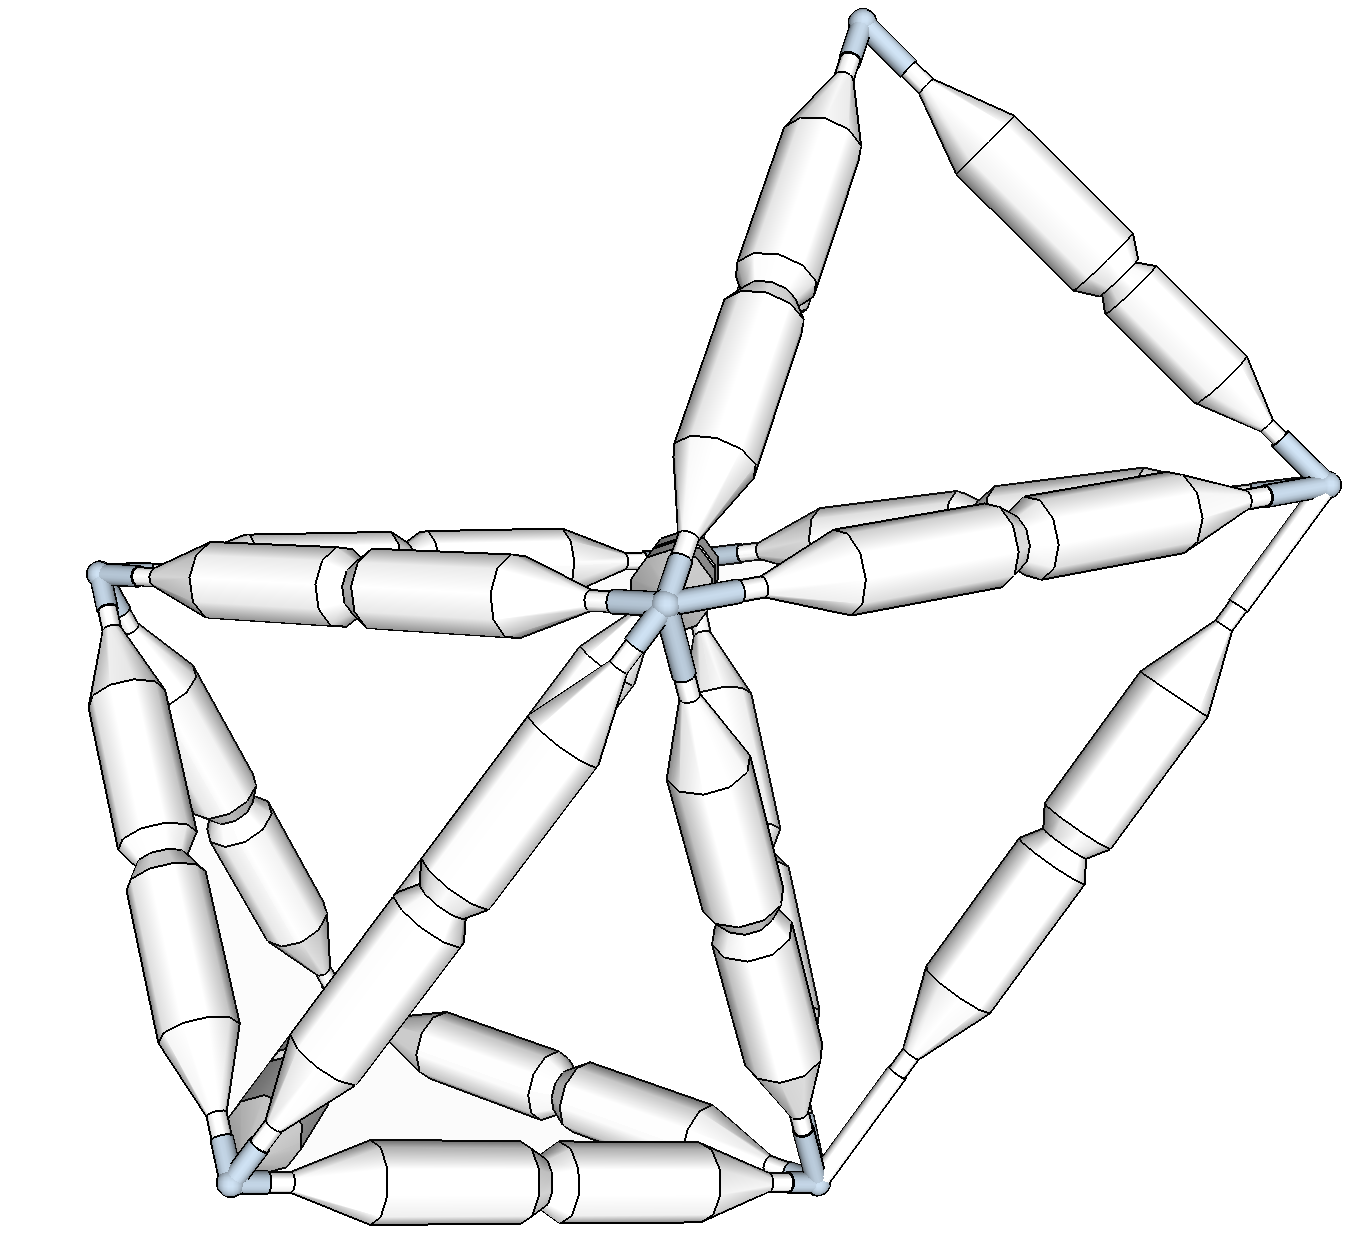
\includegraphics[height=120px]{Implementation/relax_one.png}
    \captionof{figure}{The relaxation algorithm applied with only one iteration. The extension of the lower right edge resulted in growing incident edges as well.}
    \label{fig:leg_asset}
  \end{minipage}%
  \vspace{3cm}
  \begin{minipage}[t]{5cm}
    \centering
    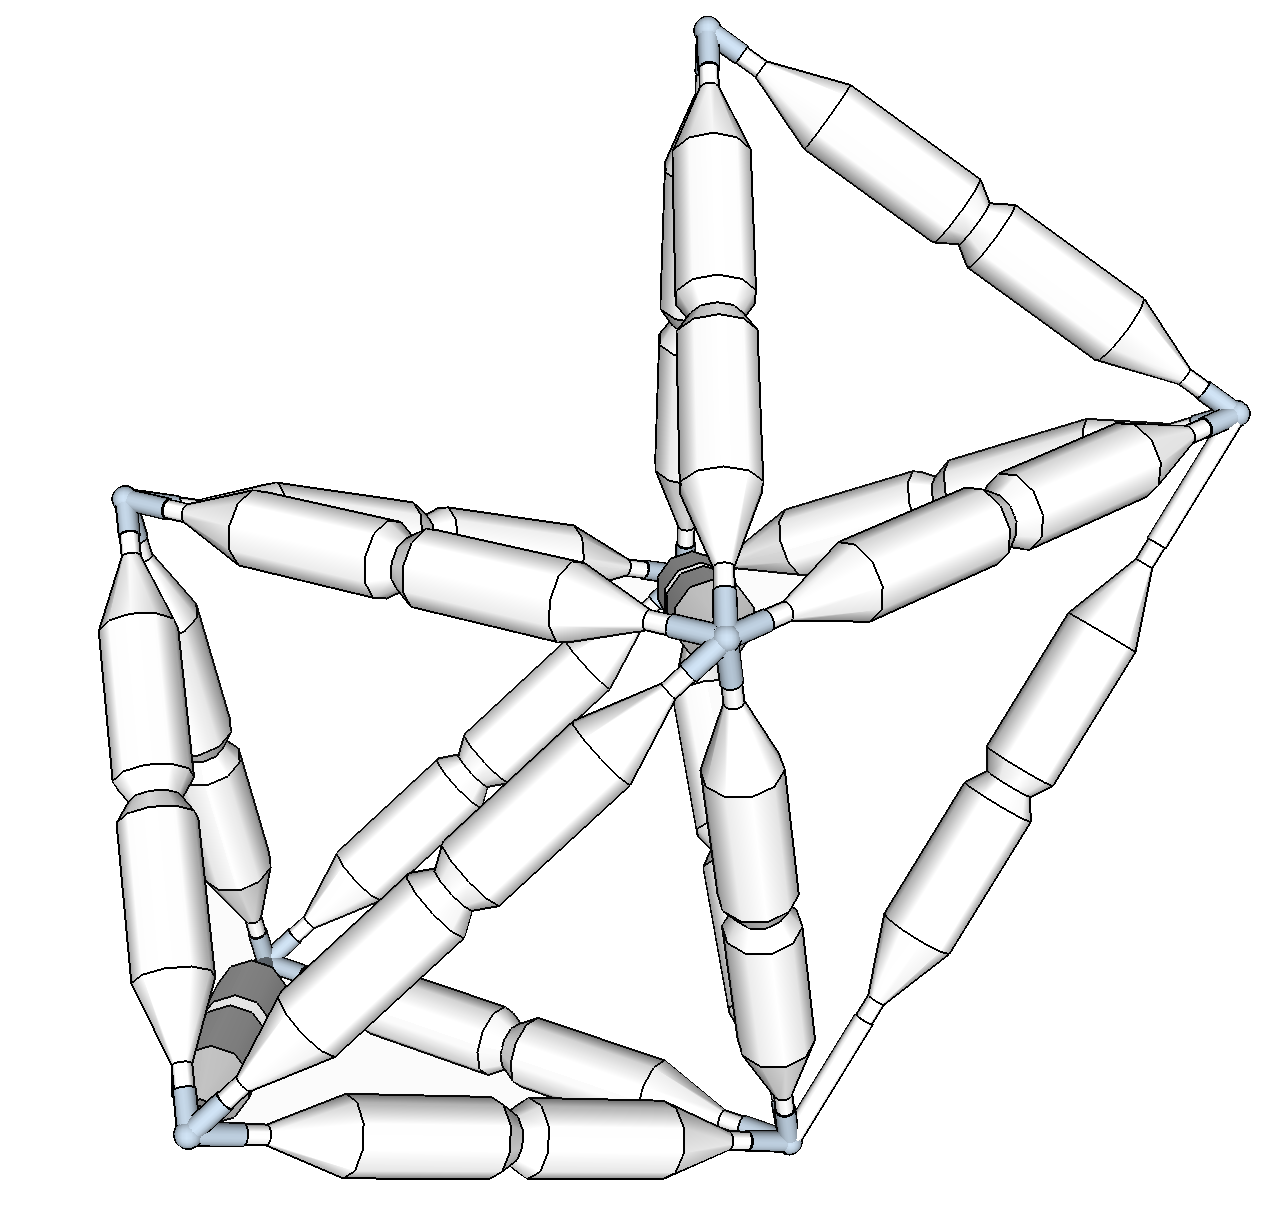
\includegraphics[height=120px]{Implementation/relax_many.png}
    \captionof{figure}{The relaxation algorithm applied with up to 20'000 iterations. Growing the lower right edge caused other nodes to translate, but the lengths of incident edges stayed the same.}
    \label{fig:spider_in_progress}
  \end{minipage}
\end{figure}

\subsection{Animation}
The animation pane is inspired by existing animation software, such as Unity\footnote{https://unity3d.com/}. It is based on so-called keyframes. A keyframe always acts on a certain piston group. It indicates the extension of all actuators in this group at a given time. Keyframes are placed on a timeline, which stretches over a set length of time. By placing keyframes on this timeline, a curve is created, which demonstrates the movement of the actuator group over this time.\\
Keyframes are positioned by using a slider and placing a vertical line at the desired point in time. The slider sets the extension of the actuator, which is interactively indicated in the editor. Pressing the \textit{Add Keyframe} button, places the keyframe with the set extension in the timeline.\\
The created animation can be played in two different modes: single and looping run. The animation will be played at a constant speed, which is coupled to the system clock. That means that one second of the animation will correlate to one second in real-time. An internal counter keeps track of the current position in the timeline at any given time and triggers a new actuator movement after passing a keyframe.\\
The speed of an actuator is determined by the distance from the current keyframe to the next and the desired change in amplitude. The y position of the keyframe can be seen as a percentage of complete extension. If the keyframe is on the top of the timeline, it has a value of 1 and each actuator in the group will be fully expanded, disregarding its length. Similarly, if the keyframe is on the bottom, its value is 0 and all actuators are fully contracted. The x value of the keyframe is also mapped in [0, 1], with 0 being the beginning of the timeline and 1 the end.
\begin{equation}
  \Delta_y = next\_keyframe.y - last\_keyframe.y\\
\end{equation}
\begin{equation}
  \Delta_x = next\_keyframe.x - last\_keyframe.x\\
\end{equation}
\begin{equation}
  v = \frac{\Delta_y * (actuator.max\_length - actuator.min\_length)}{((\Delta_x * timeline\_length) \bmod timeline\_length}
\end{equation}
The speed of an actuator is calculated by multiplying the delta of the expansion component of the last and the next keyframe with the range of motion of an actuator and dividing it by the time component of these keyframes, multiplied by the timeline length, modulo the timeline length to account for looping of the animation.\\
As actuators in a group can have different lengths, they will only receive the $\Delta_y$ value, combining it with their possible extension length and the time component. The simulation will then trigger the movement of the given actuators.

\section{Physics Simulation}\label{sec:simulation}
TrussFormer's force analysis used to be based on \textit{Finite Element Analysis}, calculated asynchronously on a remote server. This provided fairly accurate results and did not require a powerful computer to run. However, TrussFormers' responsibilities evolved during the course of its life and we decided to implement a real-time physics engine inside of our plug-in.\\
We decided to use the SketchUp plug-in \textit{MSPhysics} by Anton Synytsia\footnote{https://github.com/AntonSynytsia/}. MSPhysics is capable of calculating real-time physics on SketchUp elements and creates a customizable physics world in the modeling software. This MSPhysics world has parameters, like gravity, update timestep, and solver model which we can adapt to maximize accuracy and speed of the simulation.\\
The simulation uses the animation feature of SketchUp. A ruby class can act as a Sketchup::Animation when it implements the \textit{nextFrame} method, which must return true until the animation ends. This method is called every time SketchUp receives the signal that a new frame should be rendered. We do that by calling \textit{view.show\_frame} (s.a. listing \ref{lst:simulation}), which will trigger SketchUp to start rendering the next frame based on the simulation updates that happened earlier. We call this function as the first step in our nextFrame method, because this way, SketchUp can start rendering, while our simulation does the next physics update.\\
\begin{lstlisting}[language=Ruby, label={lst:simulation}, caption=Simulation nextFrame method]
def nextFrame(view)
    view.show_frame
    return @running unless @running && !@paused

    update_world
    update_hub_addons
    update_entities

    if (@frame % 5).zero?
      send_sensor_data_to_dialog
    end

    @frame += 1
    update_status_text

    @running
end
\end{lstlisting}
During this update, the physics engine calculates new forces on each physics component of the built object. For that, first all static forces are applied to the object. These are forces added by the \textit{Add Force Tool} or static forces calculated by the \textit{GenericPointToPoint} joints. Using these values and all other intrinsic parameters included in the physics objects, we call the entry point to our MSPhysics plug-in. The \textit{@world.advance} function calculates the change of forces and positions from one timestep to another. In our physics world, one timestep correlates to 1/60s, to achieve realistically timed results assuming that SketchUp itself runs with 60 frames per second.\\
After each world update, the tensions on each link are recorded for visualizing them later. This has to be done, because there could potentially be multiple world updates per render step and we do not want to miss crucial forces.\\
These steps in \textit{update\_world} are done for a specified number of times. In regular animation mode, one world update is calculated per frame, however some tools use the simulation in the background for static checks or other calculations. These tools do not need to display the in-between steps, so they can calculate multiple world updates back-to-back.\\
With the knowledge of the new physics calculations, we can send information about the stress level of each joint to SketchUp. We color the links depending on the tension force on them. A blue color means negative tension force, i.e. pulling force, while red color means positive force, i.e. compressing force. The higher the force, the deeper the color gets.\\
\begin{figure}[h!]
    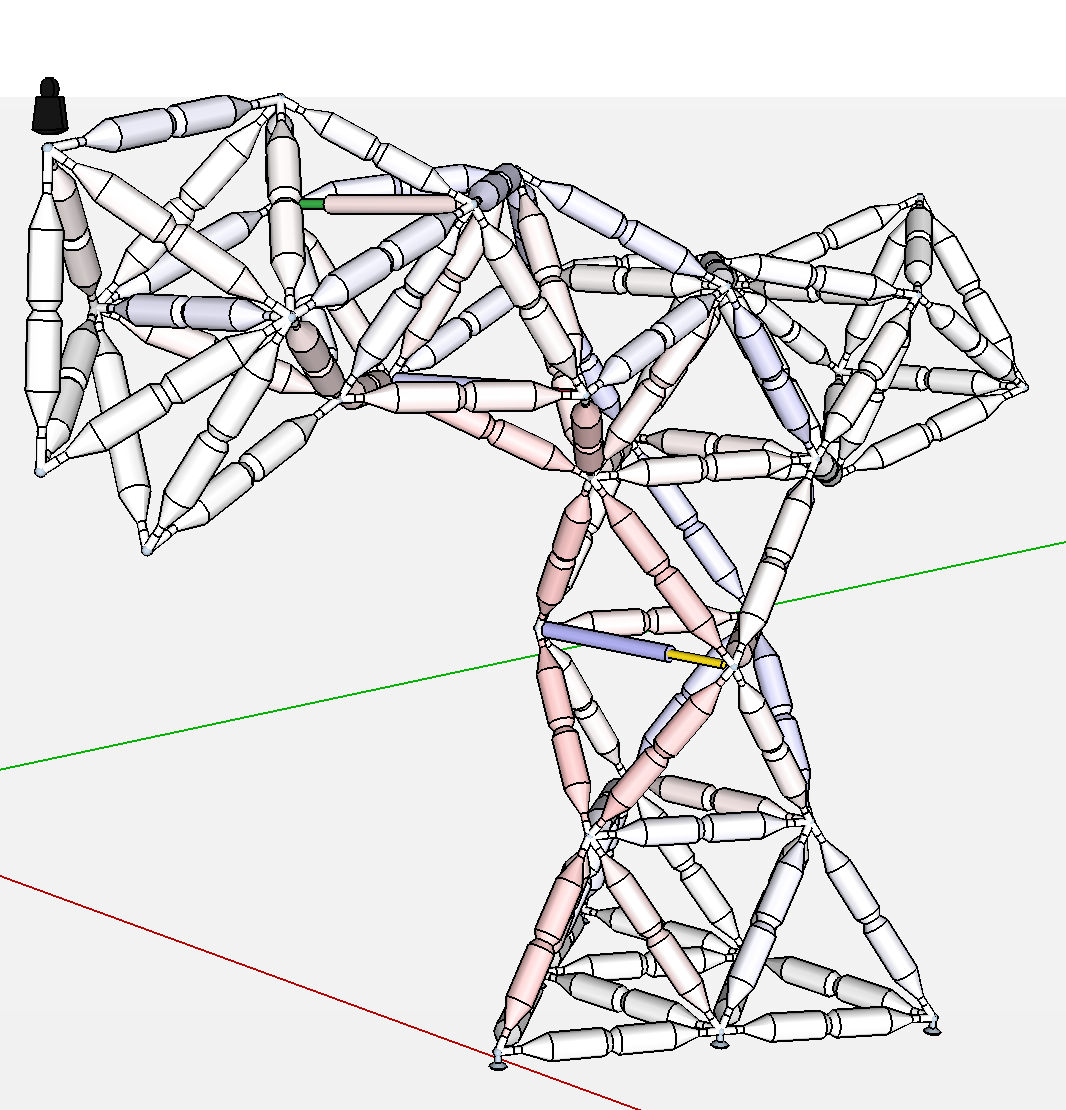
\includegraphics[width=\textwidth]{Implementation/Forces.png}
    \centering
    \caption{Visualization of forces acting on edges. Blue - tension force, red - compression force, white - little or no force}
    \label{fig:force_visualization}
\end{figure}
Once the physics portion of the rendering step is done, our own graph structure has to be updated. For that, each edge and node updates their own positions and transformations based on their internal physics objects.\\
As a last step, sensor data is send to the respective UIs in order to draw a chart depicting physical data.

\subsection{Actuators}
Actuators are implemented using the \textit{TrussFab::PointToPointActuator} joint. These joints provide position control. The \textit{controller} of the joint can be set to a length in m relative to a starting position (per default the middle position). This tells the simulation, that this joint wants to change its length to the provided value. Dependent on the speed of the joint, it will approach this position over multiple world iterations. A setting that can influence the motion of actuator joints is the damping factor, which can be set to a ratio of extension (with 0 being full contraction and 1 being full extension). The damping factor will linearly slow down the actuator starting from the set value, approaching the end with a smoother, less radical motion.

\subsection{Force Control}
Instead of position controlled joints, TrussFormer also provides joints with force control. These joints do not have a controller that can be set to a length, but a force function. The force can be set dynamically during the simulation, making force controlled joints a very flexible way to create motion.\\
Possible uses for these joints are springs. A spring exerts more force, the further it is compressed. Transferring this concept to our cylindrical links, such a spring would produce more force, the smaller the distance between two nodes is, according to the formula $F = -k * x$, with k being a spring constant, depending on the material or thickness of the spring and x being the difference between the uncompressed length of the spring (e.g. the actuator in its full extension) and its current length.

\subsubsection{PID}\label{sec:pid}
Another use case for force-controlled joints is PID controlled actuation. A proportional-integral-derivative (PID) controller is a mechanism for closed-loop control. It uses sensor values from the system, in our case the length of the actuator, and gives feedback to the control unit.\\
A PID controller will continuously calculate an error value as the difference between a desired value, e.g. the actuator position to be reached, and a current ``process variable''. The process variable is calculated as the weighted sum of the proportional, integral and derivative control terms. The controller attempts to minimize the error value by adjusting these terms.\\
The proportional term depicts a value proportional to the current error value. If the error is large, e.g. if the actuator is fully contracted, but should be fully expanded, the proportional value is large as well, telling the control unit to produce high pressure. The proportional term alone will, however, never reach the desired point, because the smaller the error value becomes, the smaller the produced pressure will be. Also it can not account for inertia of an object, as it will only produce a force in the other direction (i.e. a breaking force), if the sensor values overshot the desired position. This will create an oscillating motion around the desired position.\\
The integral part takes past error values into account, which are integrated over time. It cumulates residual error values, left behind by proportional control. If the error gets smaller, the integral term will stop growing. This will compensate the proportional term approaching zero.\\
The P and I terms will already achieve a reasonable result. The derivative term will optimize this result further. It can be seen as an estimate of the future, based on the error value's rate of change. The effect of the derivative term is that an extra control factor is included if the error rate increases and a damping factor added if the rate decreases.

\subsection{Evaluation}
We aimed to make our software simulation as accurate to the real-world object as possible. To calibrate the simulation values, we therefore measured the forces of our T-Rex example.\\
\begin{figure}[h!]
    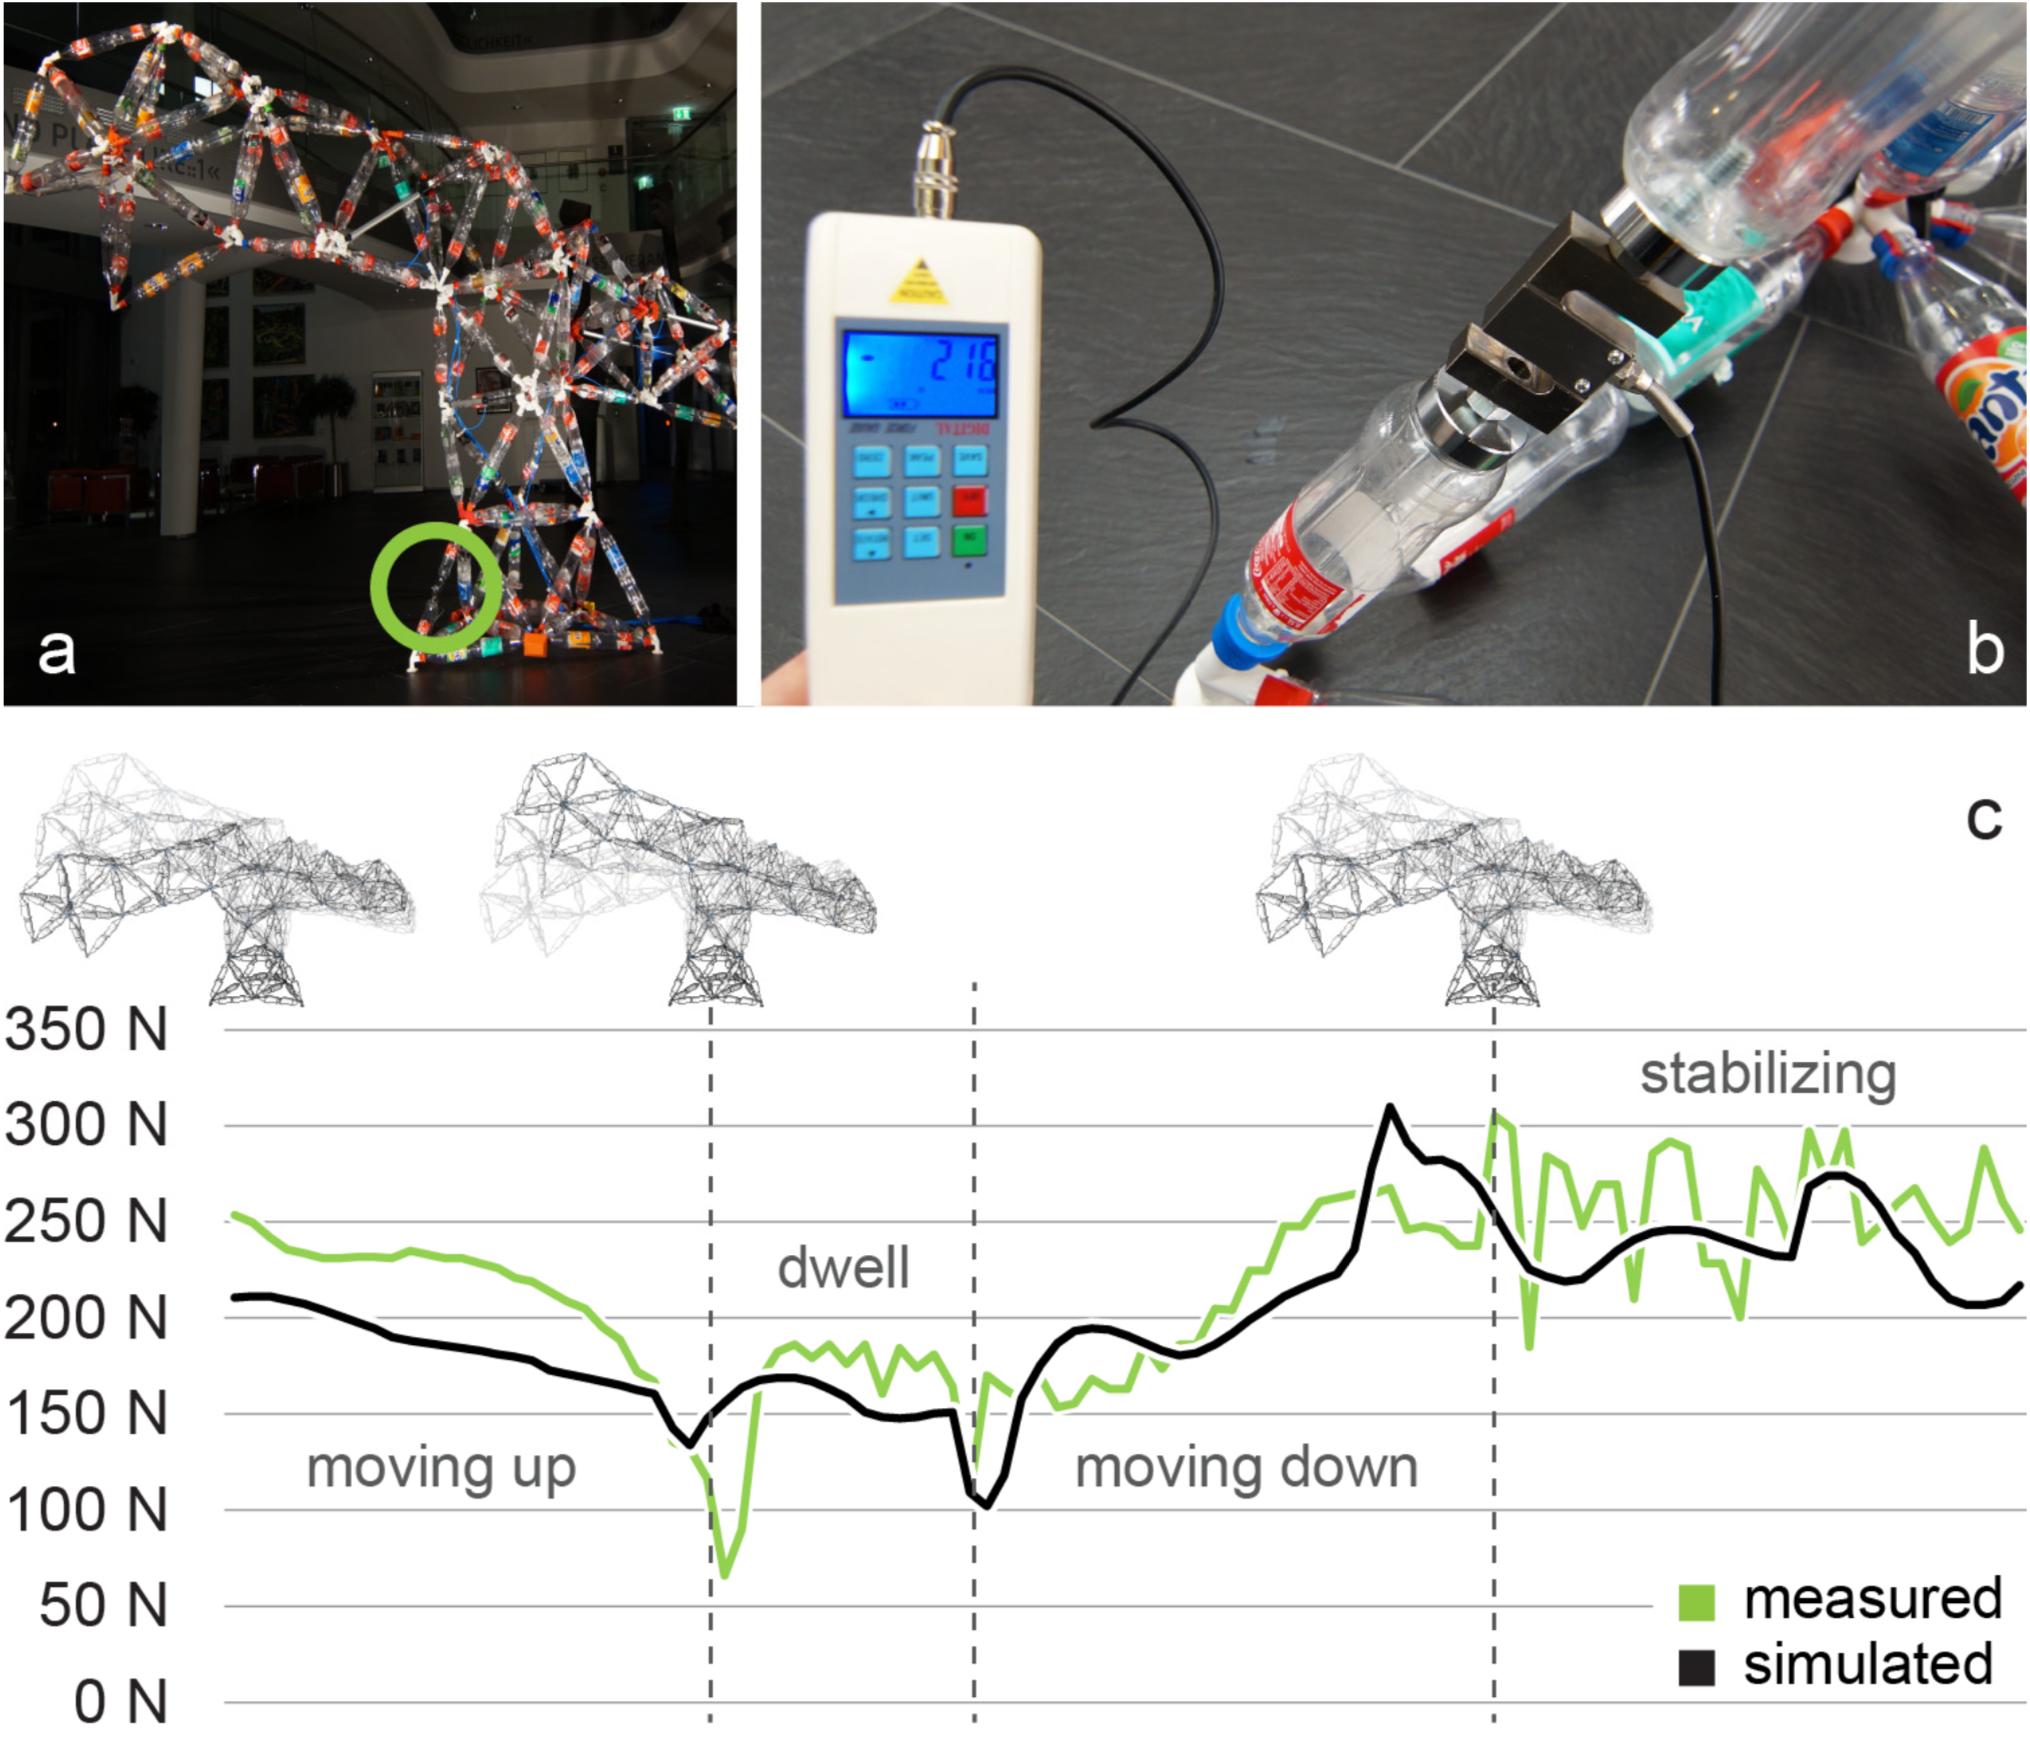
\includegraphics[width=\textwidth]{Implementation/force_measurement.png}
    \centering
    \caption{(a) We measured the forces on the bottom front edge of the T-Rex (b) using a digital force gauge. (c) The measured forces agree with the simulated forces.}
    \label{fig:force_measurement}
\end{figure}
We used a digital force sensor, with a capacity of 5000N and an error rate of 0.5\%, on the front bottom edge of the T-Rex (Figure \ref{fig:force_measurement} a-b). It was placed between two small bottles, giving the edge the same length as it would have had with two big bottles. We chose this position, because it bears the largest force due to the long lever force the neck of the T-Rex produces. Our test case consisted of moving the head up from its lowest to its highest and then back down to its lowest position again. The same movement, with the same speed, was programmed in the simulation. Figure \ref{fig:force_measurement}c shows, that both, the simulated and the measured force, are in agreement.

\section{Hinge System}
The export of 3D printable files is one of the main contributions of TrussFormer. It enables users to create their designed objects in the real world without the need to understand the complex hinge systems necessary to create the desired movements.\\
The export functionality consists of multiple steps. First, the system determines where hinges need to be placed and where static hubs are sufficient. After that, the possible motion has to be maximized. The bottles need a minimum distance to the rotation center of each hub in order to not collide with each other, to properly secure them using the cuffs and align them with the hinge movement.

\subsection{Hinge Placement Routine}\label{sec:hinge_placement_impl}
We use an empirical approach to determine the placement of hinges. Using the physics engine, we move all actuators, one after another, and measure the angular difference between adjacent triangles. If the difference exceeds a certain threshold, the common node of these two triangles needs a hinge connecting adjacent edges.\\
First, all static groups are determined. Static groups are connected structures, in which no rotation is happening, while actuators are moving.

\subsection{Minimization Logic}
In order to achieve the maximum amount of motion, while keeping the minimum amount of printing time, we created a solution for minimizing hinge and hub sizes.\\
For hinges, three lengths are of importance. These lengths consist of the distance from the rotation center to the lower side of the hinge connector (l1 distance), the height of the connector itself (l2 distance) and an optional third length being the elongation of this hinge, i.e. the length of the edge connector (l3 distance).
TODO: I am actually not sure if we do anything special here. Check this.
\begin{figure}[ht]
  \centering
  \begin{minipage}[t]{5cm}
    \centering
    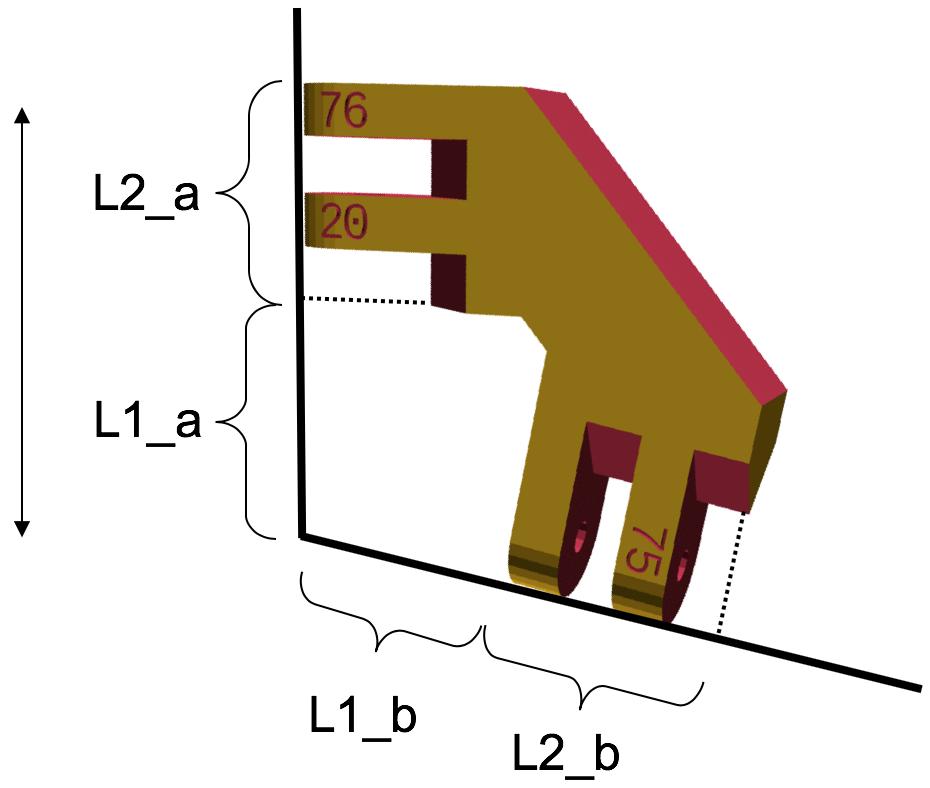
\includegraphics[height=120px]{Implementation/hinge_lengths.png}
    \captionof{figure}{L1 and L2 lenghts of a hinge part}
    \label{fig:leg_asset}
  \end{minipage}%
  \vspace{3cm}
  \begin{minipage}[t]{5cm}
    \centering
    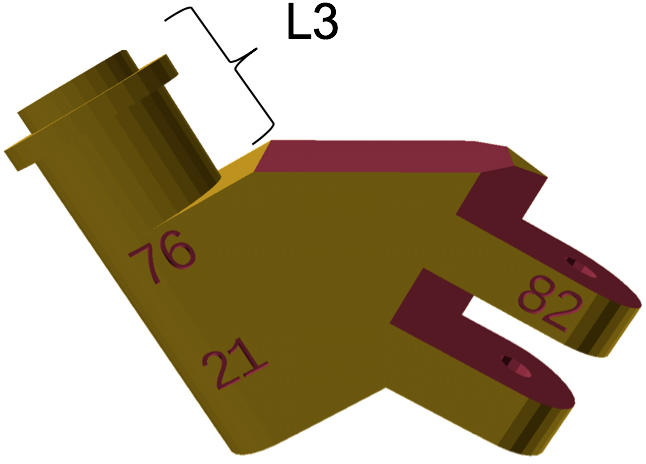
\includegraphics[height=120px]{Implementation/hinge_l3.png}
    \captionof{figure}{L3 length of a connector}
    \label{fig:spider_in_progress}
  \end{minipage}
\end{figure}
- elongates and shortens edges so that maximum movement is possible with minimum material use\\
- uses iterative relaxation algorithm, will be explained in \ref{sec:relaxation}

\subsection{Generating the 3D Models}\label{sec:openscad_impl}
In order to get printable files, our abstract description of the object has to be converted into a physical representation. To achieve this, we used a modeling language called \textit{OpenSCAD}. After optimizing the structure for the most possible movement, the resulting arrangement of nodes and edges will be transferred to OpenSCAD. OpenSCAD enables us to create 3D structures programmatically. We use it to create 3-dimensional primitives, such as spheres, cubes or cylinders, and to apply set operations, like \textit{difference} or \textit{union} on them.\\
OpenSCAD provides an editor which can be used to prototype a model. This editor, including some example operations can be seen in Figure \ref{fig:openscad_overview}. We used this editor to create the template functions used for creating the final hinge and hub models.
\begin{figure}[h!]
    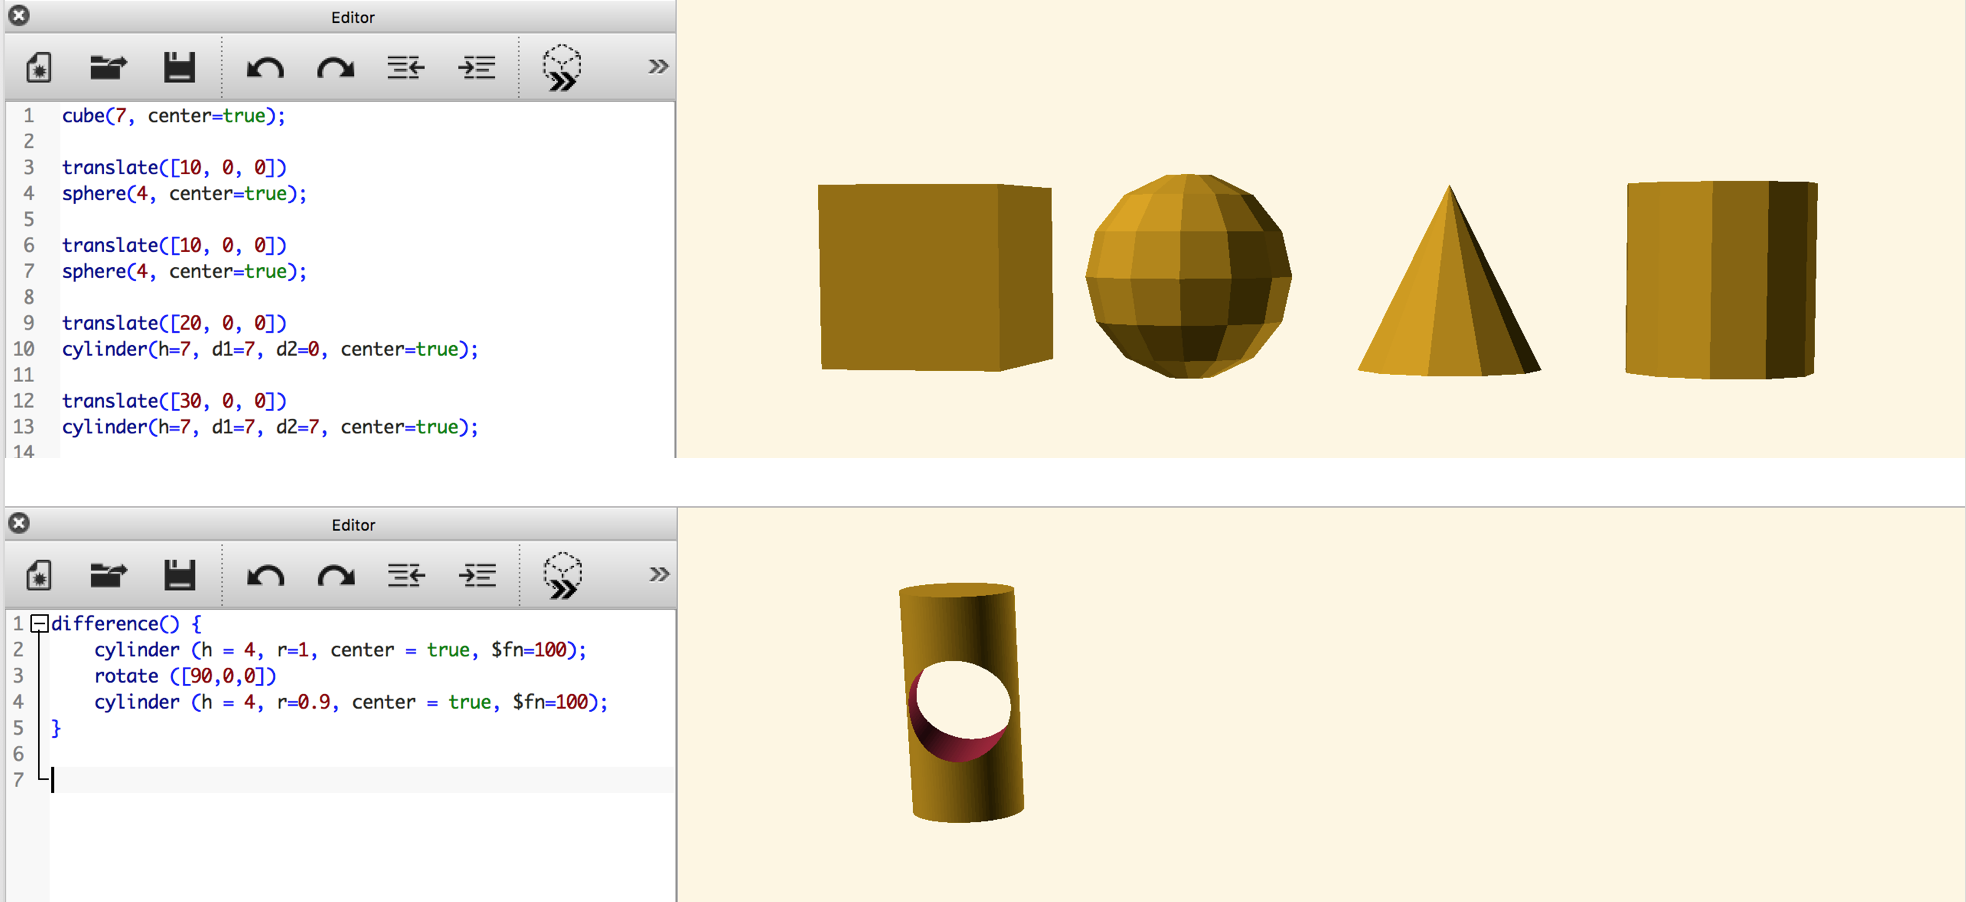
\includegraphics[width=\textwidth]{Implementation/openscad_overview.png}
    \centering
    \caption{The OpenSCAD editor containing some example code.}
    \label{fig:force_measurement}
\end{figure}
